\documentclass[border=5pt]{standalone}
\usepackage{xcolor}
\usepackage{pgfplots}
\usepackage{tikz}
\usetikzlibrary{patterns}

% Define bar chart colors
%
\definecolor{bblue}{HTML}{4F81BD}
\definecolor{rred}{HTML}{C0504D}
\definecolor{ggreen}{HTML}{9BBB59}
\definecolor{ppurple}{HTML}{9F4C7C}
\definecolor{orange}{HTML}{FF7E00}
\definecolor{yellow}{HTML}{FFFF66}

\pgfplotsset{every tick label/.append style={font=\large}}

\begin{document}
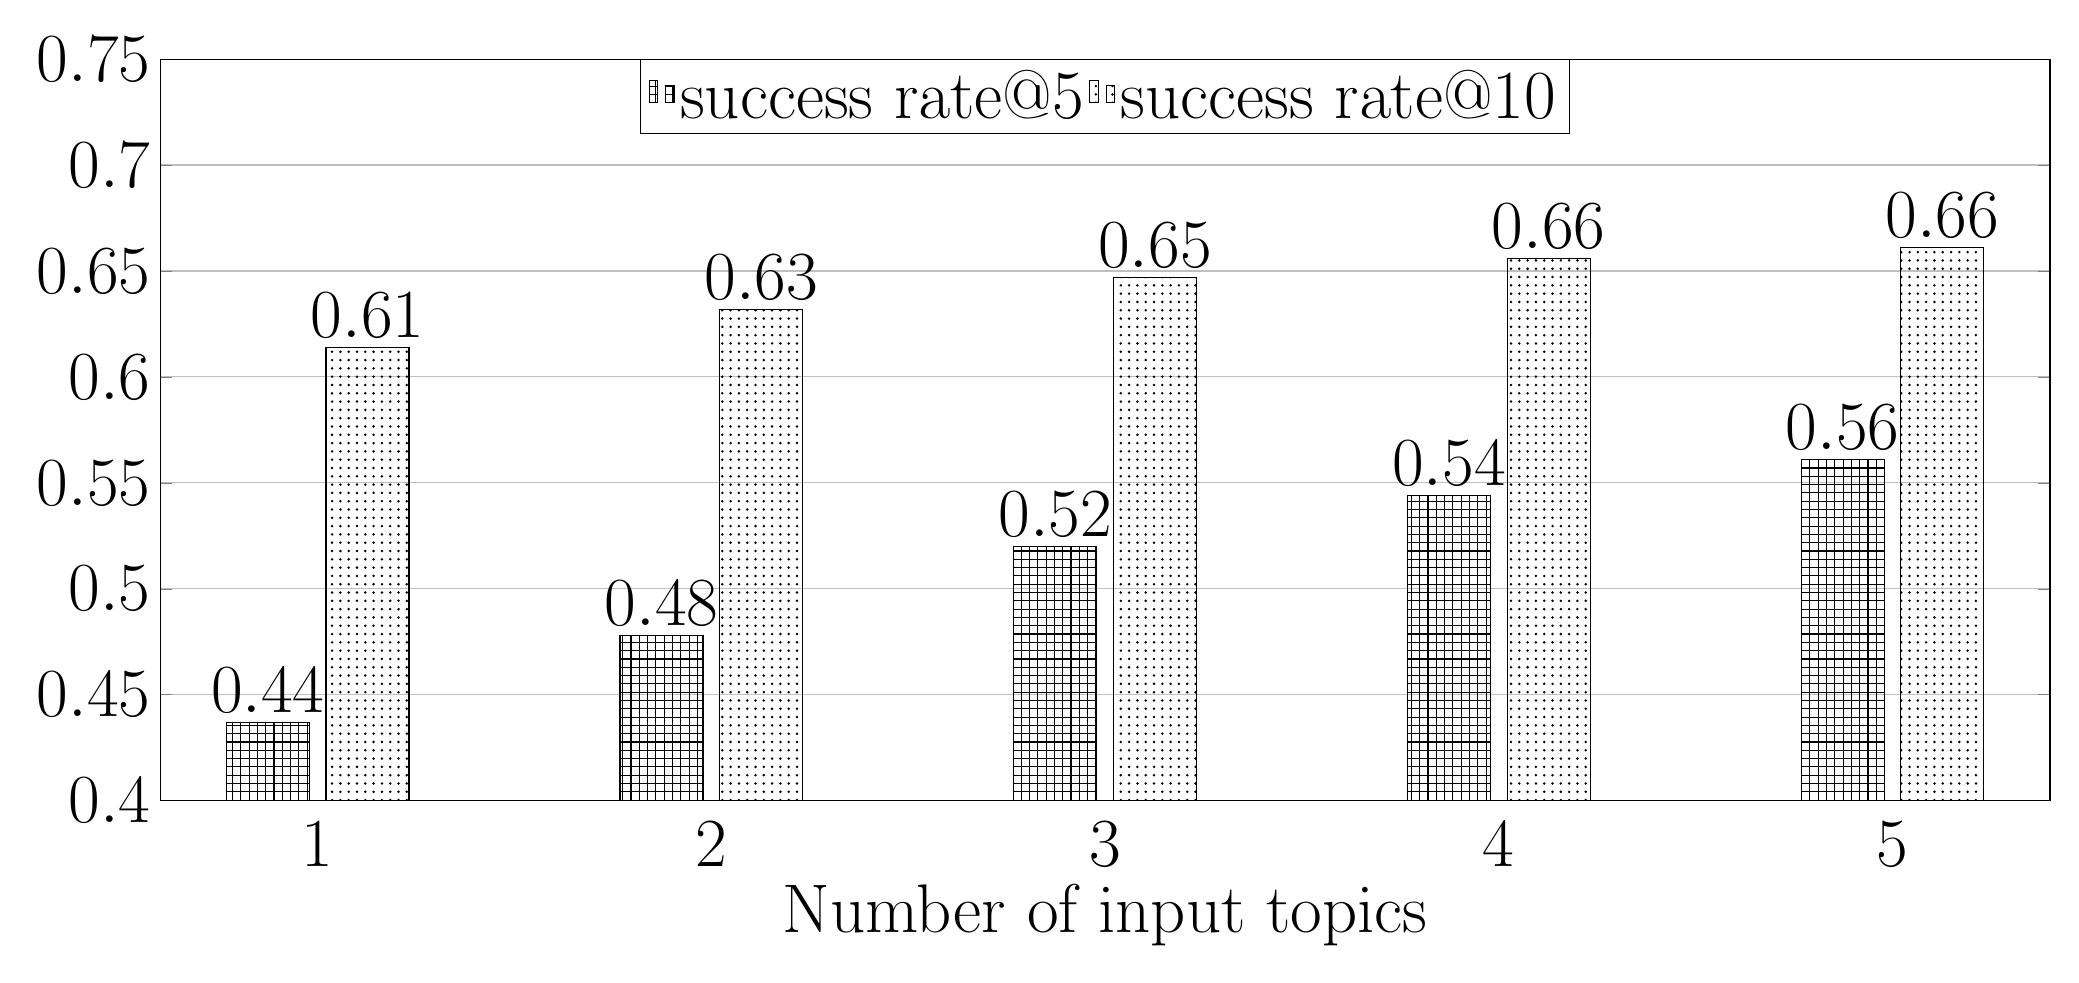
\begin{tikzpicture}
    \begin{axis}[
        width  = 6cm,%*\textwidth,
        height = 11cm,
        major x tick style = transparent,
        ybar = 6pt,
        ymin = 0.40, ymax = 0.75,
        x=5cm,
        bar width=30pt,
        ymajorgrids = true,	
        xtick = data,
        scaled y ticks = false,
%		legend style={at={(0.5,-0.1)},
%		legend style={at={(0.5,1.1)}, anchor=north,legend columns=-1,font=\small},
      	legend style={at={(0.5,1)},	anchor=north,legend columns=-1,font=\Huge,
		anchor=north,legend columns=-1},
		enlarge x limits={abs=2.0cm},
		nodes near coords,
		nodes near coords style={font=\Huge},
	    xlabel={Number of input topics},
	    xlabel style={font=\Huge, at={(axis description cs:0.5,-0.1)},},
	    every tick label/.append style={font=\Huge},
%	    ylabel = {Success rate@5 (\%)},
        symbolic x coords={1,2,3,4,5},
    ]
        \addplot[style={black,fill=bblue,mark=none,pattern=grid}]
            coordinates {(1, 0.437) (2, 0.478) (3,0.520)(4, 0.544)(5, 0.561)};
            
        \addplot[style={black,fill=orange,mark=none,pattern=dots}]
            coordinates {(1, 0.614) (2, 0.632) (3,0.647)(4, 0.656)(5, 0.661)};
                      

%      	\addplot[style={orange,fill=orange,mark=none}]
%            coordinates {(D$_1$,0.02) (10,0.902884311) (15,2.392886747)};
        \legend{ success rate@5, success rate@10}
    \end{axis}
\end{tikzpicture}
\end{document}